%%%%%%%%%%%%%%%%%%%%%%%%%%%%%%%%%%%%%%%%%
% IITG Thesis
% LaTeX Template
% Version 1.41 (22/08/14)
% Prepared According to IITG-EEE Format by:
% Gaurav Saxena
%
% Original authors:
% Steven Gunn
% http://users.ecsf.soton.ac.uk/srg/softwaretools/document/templates/
% and
% Sunil Patel
% http://www.sunilpatel.co.uk/thesis-template/

% Edited by:
% Gaurav Saxena
% 
%
% License:2
%2

% CC BY-NC-SA 3.0 (http://creativecommons.org/licenses/by-nc-sa/3.0/)
%
% Note:
% Make sure to edit document variables in the THESIS DETAILS section in this file
%
%%%%%%%%%%%%%%%%%%%%%%%%%%%%%%%%%%%%%%%%%

%----------------------------------------------------------------------------------------
%	PACKAGES AND OTHER DOCUMENT CONFIGURATIONS
%----------------------------------------------------------------------------------------

\documentclass[10pt, a4paper, oneside]{Thesis} % Paper size, default font size and one-sided paper
\usepackage{graphicx}
%\documentclass[12pt, a4paper, oneside]{Thesis} % Paper size, default font size and one-sided paper
\usepackage[T1]{fontenc}
\usepackage[utf8]{inputenc} %% for using degree symbol
\usepackage{siunitx} %% for using degree symbol \ang{90} = 90degree {\si{\degree} gives the degree symbol}
\usepackage[square, numbers, comma, sort&compress]{natbib}
\usepackage{tabularx}
\usepackage{lettrine}
\usepackage{multicol,ltablex,supertabular,latexsym}
\usepackage{amssymb,setspace,amsmath}
\usepackage{pdflscape}
\usepackage{url}
\usepackage{subcaption}
\usepackage{multirow}
\usepackage{threeparttable}
\usepackage{graphics}
\usepackage{epsfig}
\usepackage{epstopdf}
\usepackage{subfigure}
\usepackage{graphicx}
\usepackage{subfig}
\usepackage{array}
\usepackage{longtable}
\usepackage{rotfloat}
\usepackage{textcomp}
\usepackage{multirow}
\usepackage[ american]{babel}
\usepackage{comment}
\usepackage{mathtools}
\usepackage{enumitem}
\usepackage[export]{adjustbox}
%%
\usepackage{algorithm}
\usepackage{bm}
\usepackage[noend]{algpseudocode}
\usepackage{amsmath}
\DeclareMathOperator*{\argmax}{arg\,max}%%

\usepackage{morefloats}
\usepackage{verbatim}
\usepackage{mathastext} %[LGRgreek]
\usepackage{pdflscape}
\usepackage{changepage}
\usepackage{floatpag}
%\usepackage{extra_functions}

\hypersetup{urlcolor=black, colorlinks=true} % Colors hyperlinks in blue - change to black if annoying
\title{\ttitle} % Defines the thesis title - don't touch this



\makeatletter
\renewcommand{\sfdefault}{lmss}
\newcommand{\lyxmathsym}[1]{\ifmmode\begingroup\def\b@ld{bold}
  \text{\ifx\math@version\b@ld\bfseries\fi#1}\endgroup\else#1\fi}
%\newcommand{\degree}{\ensuremath{^\circ}}
%%% Because html converters don't know tabularnewline
\providecommand{\tabularnewline}{\\}


\def\hlinewd#1{%
\noalign{\ifnum0=`}\fi\hrule \@height #1 %
\futurelet\reserved@a\@xhline}

\makeatother

\begin{document}

\frontmatter % Use roman page numbering style (i, ii, iii, iv...) for the pre-content pages
%
\setstretch{1.3} % Line spacing of 1.3

% Define the page headers using the FancyHdr package and set up for one-sided printing
\fancyhead{} % Clears all page headers and footers
\rhead{\thepage} % Sets the right side header to show the page number
\lhead{} % Clears the left side page header

\pagestyle{fancy} % Finally, use the "fancy" page style to implement the FancyHdr headers

\newcommand{\HRule}{\rule{\linewidth}{0.5mm}} % New command to make the lines in the title page

% PDF meta-data

%----------------------------------------------------------------------------------------
%	THESIS DETAILS
%----------------------------------------------------------------------------------------
\newcommand{\thesisTitle}{Spoken Language Recognition}
\newcommand{\authorName}{Jagabandhu Mishra}
%\newcommand{\enrollmentNumber}{2016342002}
\newcommand{\supervisorTitle}{Prof.} %Eg: Prof. , Dr. , etc.
\newcommand{\supervisorName}{S.R.M. Prasanna} %Do not add title with the name 
%\newcommand{\degreeName}{Master of Technology}
\newcommand{\departmentName}{Electrical Engineering}
%\newcommand{\studentType}{master's student} 
%\newcommand{\studentType}{undergraduate student}
%\newcommand{\studentType}{research scholar}

%----------------------------------------------------------------------------------------
%	TITLE PAGE
%----------------------------------------------------------------------------------------
% 
% \begin{titlepage}
% \begin{center}
% 
% {\bfseries \fontsize{18}{19}\selectfont{\thesisTitle}}\\[1.5cm]
% 
% 
% %\large \textbf{A} \\ \textbf{Thesis Submitted} \\ \textbf{in Partial Fulfillment of the Requirements} \\ \textbf{for the Degree of} \\ \textbf{\expandafter\uppercase\expandafter{\degreeName}} \\ \textbf{By} \\ [1.5cm] \textbf{\expandafter\uppercase\expandafter{\authorName}}\\  \textbf{Under the Supervision of \supervisorTitle \ \expandafter\uppercase\expandafter{\supervisorName}} \\[1.5cm] % University requirement text
% 
% \large \textbf{A} \\ \textbf{M.Tech. Phase I}\\[1.5cm] \textbf{By} \\ [.5cm] \textbf{\expandafter\uppercase\expandafter{\authorName}}\\[2cm]
% 
% \includegraphics[scale=0.2]{Images/Logo_Transper} \\ [2cm]
% 
% 
% 
% \small \textbf{ DEPARTMENT OF ELECTRONICS \& COMMUNICATION ENGINEERING } \\ \textbf{National Institute of Technology Nagaland} \\ \textbf{Chumukedima,Dimapur-797103,Nagaland(INDIA)} \\[1 cm] \textbf{December, 2017}\\ [0.3cm]
% 
% 
% \end{center}
% 
% 
% 
% \end{titlepage}
% 
%
\begin{titlepage}
 \setstretch{1}
\vspace*{\fill}
\begingroup
\centering
\textbf {\Huge Assignment-02}\\ 
\textbf{\huge Restricted Boltzmann Machine (RBM)}\\
\vspace*{\fill}
\textbf{Jagabandhu Mishra \hspace{0.3} 183081002}\\
 \textbf{Seema R. K  \hspace{0.3} 173021001}\\
 \textbf{Sawan Singh Mahara \hspace{0.3} 191081003}\\
 \textbf{Akshay A. J  \hspace{0.3} 191081001}\\
 %\textbf{Himanshu Kumar Shekar \hspace{0.3} 193081005}\\
 \
\endgroup
\vspace*{\fill}

\centering
\end{titlepage}




\setstretch{1} %%% This will reduce the line spacing to 1
%----------------------------------------------------------------------------------------
% %	DECLARATION PAGE
% %	BY YOU.
% %----------------------------------------------------------------------------------------
% \clearpage % Start a new page
% 
% \pagestyle{empty} % Page style needs to be empty for this page
% 
% \begin{titlepage}
% \begin{center}
% \textsc{\textbf{\fontsize{31}{32}\selectfont{Declaration}}}\\[2.0cm] % University name
% \end{center}
% 
%  \vspace{0.5cm}
% 
% This is to certify that the thesis entitled ``\textbf{\thesisTitle}'',
% submitted by me to the \textit{Indian Institute of Technology Guwahati}, for the award of the degree of \degreeName, is a
% bonafide work carried out by me under the supervision
% of \supervisorTitle \ \supervisorName. The content of this thesis, in full or in parts, have not
% been submitted to any other University or Institute for the award
% of any degree or diploma. I also wish to state that to the best of my knowledge and understanding nothing in this report amounts to plagiarism.
% 
% \vspace{3cm}
% 
% Signed:\\ \rule[1em]{25em}{0.5pt}\\[0.1cm] % This prints a line for the signature
% \textbf{\authorName}\\
% \textbf{\departmentName,}\\
% \textbf{Indian Institute of Technology Guwahati,}\\
% \textbf{Guwahati-781039, Assam, India.}\\[2cm] \hfill{}Date:\\ \rule[1em]{25em}{0.5pt} % This prints a line to write the date
% \end{titlepage}
% 
% %----------------------------------------------------------------------------------------
% %	DEDICATION
% %----------------------------------------------------------------------------------------
% %\clearpage % Start a new page
% %\begin{titlepage}
% %\pagestyle{empty} % Page style needs to be empty for this page
% 
% % \input{Warehouse/Dedication}
% %\end{titlepage}
% 
% %----------------------------------------------------------------------------------------
% %	DECLARATION PAGE
% %	BY YOUR GUIDE.
% %----------------------------------------------------------------------------------------
% \clearpage % Start a new page
% 
% \pagestyle{empty} % Page style needs to be empty for this page
% 
% \begin{titlepage}
% \begin{center}
% \textsc{\textbf{\fontsize{31}{32}\selectfont{Certificate}}}\\[2.0cm] % University name
% \end{center}
% 
%  \vspace{0.5cm}
% 
% This is to certify that the thesis entitled ``\textbf{\thesisTitle}'',
% submitted by \authorName \ (\enrollmentNumber), a \studentType \ in the \textit{\departmentName},
% \textit{Indian Institute of Technology Guwahati}, for the award of the degree of \degreeName, is a
% record of an original research work carried out by him under my supervision
% and guidance. The thesis has fulfilled all requirements as per the
% regulations of the institute and in my opinion has reached the standard
% needed for submission. The results embodied in this thesis have not
% been submitted to any other University or Institute for the award
% of any degree or diploma.
% 
% \vspace{3cm}
% Signed:\\ \rule[1em]{25em}{0.5pt}\\[0.1cm] % This prints a line for the signature
% \textbf{Supervisor: \supervisorTitle \ \supervisorName}\\
% \textbf{\departmentName,}\\
% \textbf{Indian Institute of Technology Guwahati,}\\
% \textbf{Guwahati-781039, Assam, India.}\\[2cm] \hfill{}Date:\\ \rule[1em]{25em}{0.5pt} % This prints a line to write the date
% 
% \end{titlepage}
% 
% %----------------------------------------------------------------------------------------
% %	ACKNOWLEDGEMENTS
% %----------------------------------------------------------------------------------------
% 
% \clearpage % Start a new page
% \begin{titlepage}
% \begin{center}
% \textsc{\textbf{\fontsize{31}{32}\selectfont{Acknowledgement}}}\\[0.8cm] % University name
% \end{center}

%   

\setstretch{1}
\pdfbookmark[1]{Acknowledgments}{acknowledgments}



\begingroup
\let\clearpage\relax
\let\cleardoublepage\relax





I take the honour and privilege to express my deep sense of gratitude to my esteemed guide 
\textbf{Dr Debadatta Pati}, Assistant Professor of ECE Department, National institute of technology Nagaland
for his scholarly instructive guidance, support and continued
encouragement throughout my work.
Without our inspiring discussions on certain issues
at times, I would have never been able to complete this work.
I greatly admire his attitude
towards research, creative thinking, hard work and dedication.

I thank the Head of the Department, \textbf{Dr P. Chinnamuthu} and other faculty members for their
help and support in carrying out my work. My thanks go to \textbf{Mr. Madhusudan Singh} sir and \textbf{Krishna Dutta} sir for 
providing an excellent facility and maintaining a good ambience in the Speech processing and pattern recognition (SPPRC) lab to carry out my work.
Their friendly and helpful nature has made my work easy.

I also like to thank Department of Electronics and Information Technology (DeitY), Govt. of India for providing financial support, as my work is the part of ongoing DeitY sponsered project title "Development of Excitation Source Features Based Spoof Resistant and Robust Audio-Visual Person Identification System".

 Finally, I must express my very profound gratitude to my parents for providing me with unfailing support and continuous encouragement
 throughout my years of study and through the process of researching. This accomplishment would not have been possible without them.

\vspace{1.5cm}
\begin{center}
\noindent \begin{tabular*}{\textwidth}{@{}l@{\extracolsep{\fill}}r@{}} \textbf{}  & \textbf{Sincerely} \\ & \textbf{\authorName}  \end{tabular*}
\end{center}

\endgroup



% \end{titlepage}

%----------------------------------------------------------------------------------------
%	ABSTRACT PAGE
%----------------------------------------------------------------------------------------

% \setstretch{1.5} %% This line spacing will be used through-out the main text
% \begin{titlepage}
% \begin{center}

% \textsc{\textbf{\fontsize{31}{32}\selectfont{Abstract}}}\\[0.8cm] % University name

% \end{center}


%  

\setcounter{secnumdepth}{2}




\begingroup
%\let\clearpage\relax
%\let\cleardoublepage\relax


{\it Replay attack} is an approach for acquiring the unauthorized access to the automatic speaker verification (SV) system by using targets' pre-recorded speech. This work investigates the usefulness of linear prediction (LP) residual signal and modelling of glottal flow derivative (GFD) signal to counter replay attacks. In detecting replay signals the major clues lie in tracing the record and playback devices characteristics that dominantly reflect at low frequency regions due to loud speaker, and at high frequency regions due to two-stage A/D conversions. In that direction, must of the attempts try to derive the discriminative feature directly from the speech signal. In signal processing terms, the speech signal can be represented as the response of a slow time-varying vocal-tract system excited by a fast time-varying impulse like excitation source. Due to the presence of vocal tract resonances, the playback device characteristics may distort more to the spectral patterns of impulse like excitation signal then the spectral pattern of speech signal. Based on the distribution nature of the mel-scale that tightly spaced in low frequency regions and reverse in inverse mel-scale, residual mel-frequency cepstral coefficients (RMFCC) and residual inverse mel-frequency cepstral coefficients (RIMFCC) features are derived from LP residual signal and glottal flow derivative mel frequency cepstral coefficients (GFDMFCC) are derived from GFD signal. The effectiveness of these features are demonstrated on ASVspoof2017 database.

In terms of equal error rate (EER), RMFCC features provide the best performance of 14.57\% and RIMFCC of 15.35\%. The fusion of RMFCC and RIMFCC features improves the performance to 10.14\%, that is comparatively better than the state-of-the-art spectral centroid magnitude coefficients (SCMC) feature performance of 11.49\% and constant Q cepstral coefficients (CQCC) of 15.12\%. The fusion of RMFCC, RIMFCC with CQCC and SCMC further improves the performance to 8.72\%. Further, the GFD signal based GFDMFCC provides an EER of 20.53\%. The fusion of GFDMFCC with CQCC and SCMC provides an EER of 8.18\%. These outcomes demonstrate the usefulness of excitation source information for developing countermeasures to replay attacks. 

% 
% {\it Replay attack} is an approach for acquiring the unauthorized access to the automatic speaker verification (SV) system by using targets' pre-recorded speech. 
% %The extended reserach works over last few decades on SV, made the voice biometrics technology considerably mature, efficient, convenient and low-cost solution. To make the SV systems publicly available for widespread comercial applications, the security of such systems must be guaranteed. The SV systems are  more vulnerable to replay attacks, as it is very easy to create, no signal processing knowledge require, only require a high quality record and replay device, which can be easily available at nominal price. This attracts the research community to develop countermeasures to replay attacks. 
% In detecting replay signals the major clues lie in tracing the record and playback devices characteristics that dominantly reflect at low frequency regions due to loud speaker, and at high frequency regions due to two-stage A/D conversions. In that direction, must of the attempts try to derive the discriminative feature directly from the speech signal. From the speech production point of view, a voiced speech signal is the output of slow time varying vocal tract system, excited by a fast time varying impulse like signal. Due to the presence of vocal tract resonances, the playback device characteristics may distort more to the spectral patterns of impulse like excitation signal then the spectral pattern of speech signal. In this work, we investigates the usefulness of linear prediction (LP) residual signal and modelling of flow derivative (GFD) signal to counter replay attacks. Based on the distribution nature of the mel-scale that tightly spaced in low frequency regions and reverse in inverse mel-scale, residual mel-frequency cepstral coefficients (RMFCC) and residual inverse mel-frequency cepstral coefficients (RIMFCC) features are derived from LP residual signal and glottal flow derivative mel frequency cepstral coefficients (GFDMFCC) are derived from GFD signal. The effectiveness of these features are demonstrated on ASVspoof2017 database.
% 
% %The initial study is made on deciding the suitable prediction order. 
% In terms of equal error rate (EER), RMFCC features provide the best performance of 14.57\% and RIMFCC of 15.35\%.
% %from $10^{th}$ order LP analysis. 
% %These results show that residual signals effectively capture the low frequency distortions with higher order LP analysis and vice versa. The higher performance in case of RMFCC features may due to the significant distortion from loud speakers. 
% The fusion of RMFCC and RIMFCC features improves the performance to 10.14\%, that is comparatively better than the state-of-the-art spectral centroid magnitude coefficients (SCMC) feature performance of 11.49\% and constant Q cepstral coefficients (CQCC) of 15.12\%. 
% %The fusion of RMFCC and RIMFCC features together with SCMC provides 9.54\% and with CQCC provides 9.34\%. Finally, 
% The fusion of RMFCC, RIMFCC with CQCC and SCMC further improves the performance to 8.72\%. Further, the GFD signal based GFDMFCC provides an EER of 20.53\%. 
% %The fusion of GFDMFCC with CQCC provides 9.23\% and with SCMC provides 9.85\%. Finally 
% The fusion of GFDMFCC with CQCC and SCMC provides an EER of 8.18\%. 
% %The results demonstrate that, even if the performance of GFDMFCC is poor but the overall performance improved when combine with state of the art speech based features. 
% These outcomes demonstrate the usefulness of processing LP residual signals and modelling of GFD signals to counter replay attacks.
% 
% 
% 
% 
% 
% 
% This observation shows, the feature derived from speech signals have contained more complementary information with the features derived from GFD signals then the features derived from LP residual signal. 
% 
% 
% 
% 
% 
% 
% 
% Automatic speaker verification (ASV) is a task of validating the claimed identity through machine by using the information available in claimants speech samples. The extended reserach works over last few decades on speaker verification technology made the Automatic speaker verification (ASV) considerably mature,efficient, convenient, low-cost and reliable solution to biometric person authentication. ASV technology is finding its way into a growing array of commercial products and services. The ASV systems are often employed for remote access (without humans supervision), or through telephone channel, provoke the chance of spoof attacks, where an impostor can immitate any target by providing later’s false speech samples. Spoofing can be done in four ways like impersonation, voice conversion, speech synthesis and replay attacks. Replay attack is very easy to create, no signal processing knowledge require, only require a high quality record and replay device, which can be easily available at nominal price. This attracts the research community to develop countermeasures to replay attacks. In detecting replay signals the major clues lie in tracing the record and playback devices characteristics that dominantly reflect at low frequency regions due to loud speaker, and at high frequency regions due to two-stage A/D conversions. Unlike speech, the spectral pattern of the impulse-like linear prediction (LP) residual signal is spread across entire frequency range, and so conjectured to be more useful. Based on the distribution nature of the mel-scale that tightly spaced in low frequency regions and reverse in inverse mel-scale, residual mel-frequency cepstral coefficients (RMFCC) and residual inverse mel-frequency cepstral coefficients (RIMFCC) features are used as the representative features.
% 
% 
% 
% 
% In that direction most of the attempts try to capture the trace of the playback device characteristics by using spectral related information, that remain almost intact in replay signals, due to the presence of high energy formants, resulting higher error in replay attacks detection task. In this work, we explore the use of linear prediction (LP) residual signal and glottal flow derivative (GFD) signals to counter replay attacks. The LP residual obtained by substracting the dominant energy (Resonances) from the speech signal and the GFD signal is obtained from the speech signal by deconvoling the vocal tract system responce using complex cepstrum decomposition method. 
% 
% In detecting replay signals the major clues lie in tracing the record and playback devices characteristics that dominantly reflect at low frequency regions due to loud speaker, and at high frequency regions due to two-stage A/D conversions. Unlike speech, the spectral pattern of the impulse-like linear prediction (LP) residual signal is spread across entire frequency range, and so conjectured to be more useful. Based on the distribution nature of the mel-scale that tightly spaced in low frequency regions and reverse in inverse mel-scale, residual mel-frequency cepstral coefficients (RMFCC) and residual inverse mel-frequency cepstral coefficients (RIMFCC) features are used as the representative features.
% 
% 
% 
% We observed that, as compared to spectral related vocal-tract features, the parametric representation of the LP residual and GFD signals shows relatively more robustness against replay attacks. Based on the distribution nature of the mel-scale that tightly spaced in low frequency regions and reverse in inverse mel-scale, residual mel-frequency cepstral coefficients (RMFCC) and residual inverse mel-frequency cepstral coefficients (RIMFCC) features are used as the representative features. The effectiveness of these features is demonstrated on ASVspoof2017 database.
% 
% The initial study is made on deciding the suitable prediction order. In terms of equal error rate (EER), RMFCC features provide the best performance of 14.57\% from $20^{th}$ order LP analysis and RIMFCC of 15.35\% from $10^{th}$ order LP analysis. These results show that residual signals effectively capture the low frequency distortions with higher order LP analysis and vice versa. The higher performance in case of RMFCC features may due to the significant distortion from loud speakers. The fusion of RMFCC and RIMFCC features further improves the performance to 10.14\%, that is comparatively better than the state-of-the-art spectral centroid magnitude coefficients (SCMC) feature performance of 11.49\%. Finally, the fusion of RMFCC and RIMFCC features together with SCMC provides 9.54\%. These outcomes demonstrate the usefulness of processing LP residual signals to counter replay attacks.
% 
% 
% In future, we aim to model the LP residual
% signal explicitly and develop countermeasures to playback
% attacks
% 
% 
% 
% the SV system an acceptable authentication system for public use, like voice biomatrics used to authenticate
% bank transactions. The SV systems are often employed for remote access (without humans supervision), or through
% telephone channel, provoke the chance of spoof attacks, where an impostor can immitate any target by providing
% later’s false speech samples. The present work deals with developing spoof resistant SV system. Spoof attacks can be
% possible in four ways, i.e. impersonation, record and replay, speech synthesis and voice conversion. A study on threat
% accessement reveals that spoofing through playback attacks is easily accessible and provoke higher false acceptance
% rate, encouraging the researchers for giving wider attention. Althogh, successful methods have been proposed in
% literature, but the reliability of the SV system against playback attacks still remains a concern. In this work we
% aim to find a well discriminative feature to distinguish the playback signal by using signal
% processing knowledge. In this work we explore the use of linear prediction (LP) residual signal with proper LP order to detect the playback attacks.
% 
% We observed that, as compared to spectral related vocal-tract features, the parametric representation of the LP residual signal
% shows relatively more robustness against playback attacks. On ASVspoof2017 database using residual inverse mel filter cepstral
% coefficients(RIMFCC) with 10 LP order gave an EER of 7.18 in development set and an EER of 16.20 in evaluation set. When
% RIMFCC is combined in feature level with conventional residual mel filter cepstral coefficients(RMFCC) with 10 LP order gave
% an EER of 11.01 in development set and an EER of 10.81 in evaluation set. Hence the features derived from LP residual with
% proper LP order can be very much useful to detect playback signals.
% 


\endgroup



% \end{titlepage}
% \cleardoublepage{}
% \setstretch{1} %%% This will reduce the line spacing

%----------------------------------------------------------------------------------------
%	LIST OF CONTENTS/FIGURES/TABLES PAGES
%----------------------------------------------------------------------------------------

\pagestyle{fancy} % The page style headers have been "empty" all this time, now use the "fancy" headers as defined before to bring them back

%\lhead{\emph{Contents}} % Set the left side page header to "Contents"
\tableofcontents % Write out the Table of Contents

%\lhead{\emph{List of Figures}} % Set the left side page header to "List of Figures"
\listoffigures % Write out the List of Figures

%\lhead{\emph{List of Tables}} % Set the left side page header to "List of Tables"
%\listoftables % Write out the List of Tables
%\lhead{\emph{Clustering Algorithms}} 

%----------------------------------------------------------------------------------------
%	THESIS CONTENT - CHAPTERS
%----------------------------------------------------------------------------------------

\mainmatter % Begin numeric (1,2,3...) page numbering

\pagestyle{fancy} % Return the page headers back to the "fancy" style

% Include the chapters of the thesis as separate files from the Chapters folder
% Uncomment the lines as you write the chapters
%



\chapter{Introduction}
\chaptermark{ Introduction}
\HRule \\[-0.5cm] % Horizontal line

\label{Chapter1} % For referencing the chapter elsewhere, use \ref{Chapter1}

\lhead{\emph{\textbf{Chapter1:} Introduction}} % This is for the header on each page - perhaps a shortened title
 
%----------------------------------------------------------------------------------------
%	SECTIONS
%----------------------------------------------------------------------------------------





\begin{spacing}{1.5}
\section{Evolution: Feedback Neural Network to Restricted Boltzmann Machine}
%\subsection{Background}
Neural networks can be used for various tasks right from pattern storage to pattern classification with appropriate selection of weights and network topology/architecture. \\
%%=====================================================================
\subsection{Feedback Neural Network and its limitations}
Feedback neural network~(FBNN) are a class of neural networks where the output of each processing unit/neuron acts as input to all other processing units and to itself. The amount of information that acts as input to the units is weighted by the strength of the link between the units. By choosing appropriate parameters for this network it can be used to perform tasks like auto-association. \\
The main goal of auto-associative networks is to learn the pattern associated with input in training phase and recall the pattern when erroneous or noisy version of input is fed to the network during the testing phase i.e. it should possess accretive behavior. If the processing units in the FBNN are linear this behavior cannot be achieved as an erroneous input will lead to the generation of erroneous output instead of pattern recall. This drawback can be overcome by replacing the linear processing units with non-linear processing units. Hence, the FBNN with non-linear processing units can be used for the task of pattern storage.  \\
The task of pattern storage involves learning the features and spatial relationship between the features associated with the input with the aim of recollecting the exact input pattern when an approximate version of the pattern is provided as input to the network. 
If we consider the output (depends on weights and biases) of each unit as energy of that unit/state, the path that state traverses in the energy landscape (energy as a function of state)  at successive instants of time can be termed as the trajectory of that sate.  The trajectory is determined by the activation dynamics model used for the network. \\
When an input is applied to the network, the activation dynamics is applied to input continuously till it reaches an equilibrium state. Theses equilibrium states are the minimum energy points explored to store the patterns in the network during the pattern storage task. It is the presence of these energy minima’s that help in pattern retrieval when an approximate version of input is fed to the network. \\
The two parameters that need to be evaluated in FBNN are error in recall and the capacity of the network.
The error in recall occurs when the network recollects a wrong pattern when fed with noisy input. This can reduced by adjusting the weights of the network to ensure that the energy landscape of the network matches the probability distribution of the pattern to be stored.
Capacity of the network is defined as the number of patterns a network can store. It depends on the number of processing units available in the network. If the network has $N$ binary processing units, though it can have $2^N$ states, the network can store only $N$ binary patterns as the network will have only $N$ minimum energy states. Hence, the capacity of the network is determined by the number of processing units and their interconnections in the network. \\
If the number of patterns to be stored are more than the number of energy minima’s it is a hard problem and if the number of minima’s are more than the number of patterns to be stored there will be increase in false wells which in turn leads to increase in error in recall.
%To overcome the hard storage problem and reduce the error in recall Hopfield model was introduced.\\

%%=====================================================================
\subsection{Hopfield Model}
Hopfield model is a fully connected~(FC) FBNN with symmetric weights and no self-loop. The weights are updated asynchronously and the energy associated with each of the state reduces or remains same as the state of the network changes. The number of patterns to be stored is limited and is of the order of number of units.\\
Based on the rule used to update the states and output function of each unit, the Hopfiled Model can be continuous or discrete.
Discrete Hopfield model the state update is synchronous and the output function can be binary/bipolar whereas in a continuous Hopfield model the states are updated by activation dynamics and output function is continuous and non-linear.

%%=====================================================================
%\subsection{Hard Problem: Need of Hidden units and Stochastic update}
\subsection{Boltzmann machine and Restricted Boltzmann machine}
In Boltzmann machine, the errors in recall due to false minima is resolved by updating the states stochastically and asynchronously. Also, the probability distribution of patterns are considered while designing the energy minima so that the given patterns correspond to the lowest energy minima in the network. \\
The hard problem in the pattern storage task is handled by introducing additional units in the feedback network called hidden units. The units where input is applied are called visible units.

Though the Boltzmann machine appear to solve the pattern storage problem they are slow and difficult to train. Hence, Restricted Boltzmann machine was introduced. Restricted Boltzmann machines do not have connection in between the units of the same layer. Hence, easier to train as compared to Boltzmann machine.
% \section{Summary}
\end{spacing} 





\chapter{Restricted Boltzmann Machine (RBM)}
%\chaptermark{Acoustic feature extraction and classification techniques used for Spoken language recognition}
\HRule \\[-0.5cm] % Horizontal line

%\label{Chapter2} % For referencing the chapter elsewhere, use \ref{Chapter1}

\lhead{\emph{\textbf{Chapter2:} RBM}} % This is for the header on each page - perhaps a shortened title

%----------------------------------------------------------------------------------------
%	SECTIONS
%----------------------------------------------------------------------------------------
\begin{spacing}{1.5}
\section{RBM}
Restricted Boltzmann machine (RBM) is the restricted version of stochastic neural network called Boltzmann machine. Boltzmann machine is a feedback network with hidden units that supports stochastic updates (refer Fig.~\ref{fig:FBNN_n_BM}). Feedback networks are designed to solve pattern storage problems, later it extends to solve other pattern recognition tasks. Feedback networks were proposed to mimic the characteristics of biological neurons. Unfortunately, due to many computational and analytical limitations it ended with Boltzmann machines~\cite{yegnanarayana2009artificial}, after observing that Boltzmann machines need a large amount of training data and computational resources. Parallely, different types of statistical modelling techniques evolved that provide far better performance using comparatively less resources than the Boltzmann machines ever did. One such solution proposed that RBM should run by removing the interconnections between the visible units and the hidden units(refer Fig.~\ref{rbm}). 

\begin{figure}[h]
    \centering
    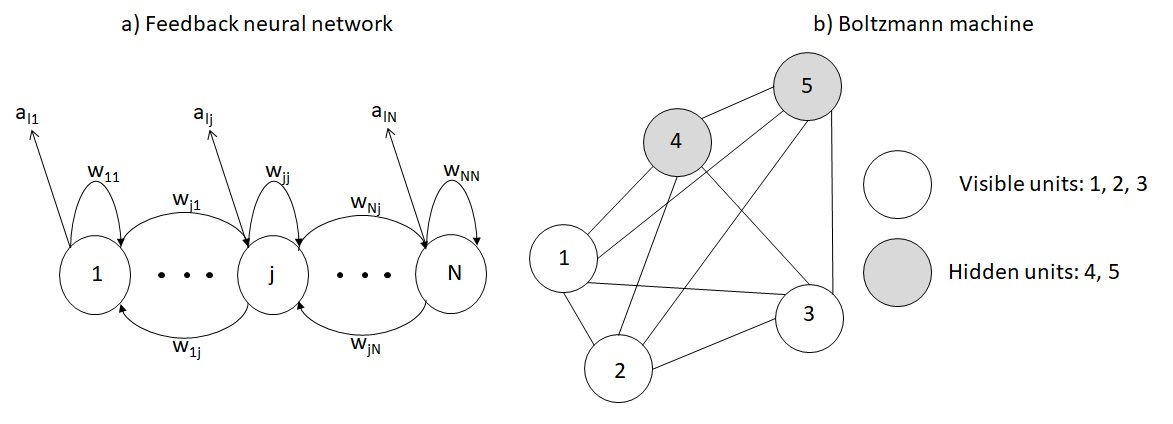
\includegraphics[scale=0.7]{Chapters/Figures/Figure_1_horizontal.jpg}
    \caption{Network architectures a) Feedback neural network b) Boltzmann machine}
    \label{fig:FBNN_n_BM}
\end{figure}

\begin{figure}[h]
    \centering
    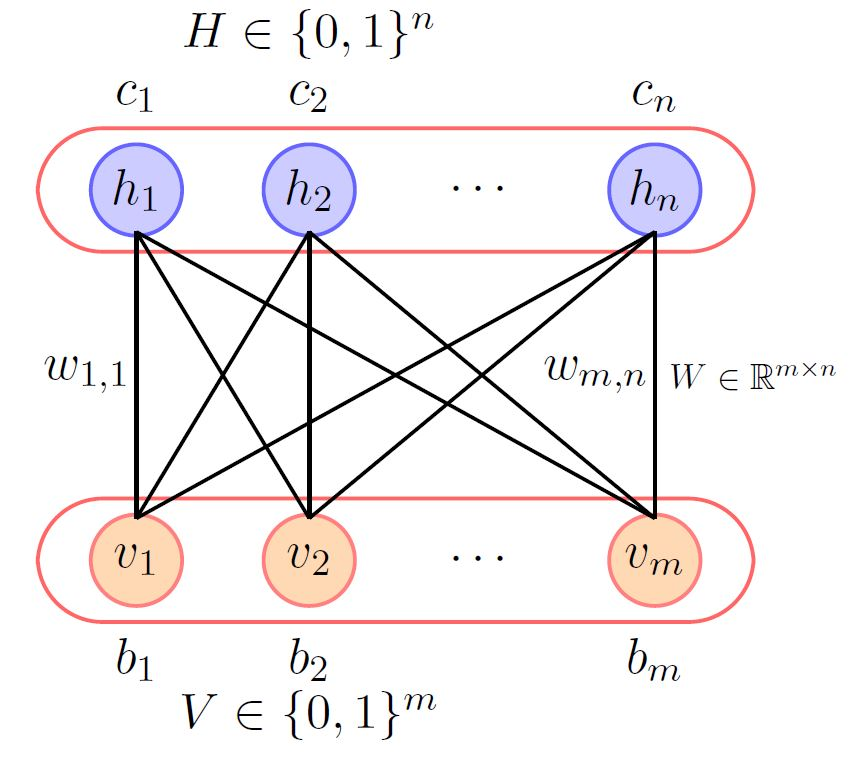
\includegraphics[scale=0.70]{Chapters/Figures/lect_19_slide_43_RBM.JPG}
    \caption{RBM}
    \label{rbm}
\end{figure}





From the feedback network, we can write the equation of energy corresponding to a given state as:
\begin{equation}
    E(V,H)=-\sum_{i}\sum_{j}w_{ij}v_{i}h_{j}-\sum_{i}b_{i}v_{i}-\sum_{j}c_{j}h_{j}
\end{equation}

and the probability of a visible and hidden unit state can be given as:
\begin{equation}
    P(V,H)=\frac{e^{-E(V,H)}}{\sum_{V}\sum_{H}e^{-E(V,H)}}
\end{equation}
where  $V \in \{0,1\}^{m}$, $H \in \{0,1\}^{n}$  for a binary RBM or $V \in R^{m}$, $H \in R^{n}$ for a continuous RBM , m and n is the number of visible and number of hidden units respectively. 
\section{RBM Training}
The training in RBM is unsupervised. Given the data points X as input to the visible units, we have to learn $P(V,H)$ which is parameterized as $ P(V,H)=\frac{e^{-E(V,H)}}{\sum_{V}\sum_{H}e^{-E(V,H)}}$, where the hidden units are unknown. 

As we want to store the pattern $X \in V$ in the network, we have to capture $P(X)$, which can be written as $\sum_{H}P(V,H)$.

So, for a given dataset D ($D=\{x_{1}, x_{2}, ..., x_{l}\}$), we have to maximize $\prod_{i=1}^{l}P(x_{i}|\theta)$, where $\theta$ are the parameters ($w_{ij},c_{i},b_{j}$) of the neural network. 

The objective function can be written as
\begin{equation}
 \begin{aligned}
 ln L(\theta)=&ln \prod_{i=1}^{l}P(x_{i}|\theta)\\
            =&\sum_{i=1}^{l}ln P(x_{i}|\theta)\\
            =&\sum_{i=1}^{l} ln P(V_{i}|\theta)\\
            =&\sum_{i=1}^{l} ln \sum_{H}\frac{e^{-E(V,H)}}{\sum_{V}\sum_{H}e^{-E(V,H)}}
 \end{aligned}
\end{equation}

we have to maximize $ln (L(\theta))$ i.e
$\max_{\theta}\sum_{i=1}^{l} ln \sum_{H}\frac{e^{-E(V,H)}}{\sum_{V}\sum_{H}e^{-E(V,H)}} $. 

We can use stochastic gradient approach to update the parameters of the network, which will maximize the objective function, for that we have to compute $\frac{\partial ln L(\theta)}{\partial \theta}$.
\begin{equation}
    \begin{aligned}
    \frac{\partial ln L(\theta)}{\partial \theta}=&\frac{\partial }{\partial \theta}
    \big[ln \sum_{H}e^{-E(V,H)}-ln \sum_{V,H}e^{-E(V,H)}\big]\\
    =&-\sum_{H}\frac{e^{-E(V,H)}}{\sum_{H}e^{-E(V,H)}}\frac{\partial E(V,H)}{\partial \theta}+\sum_{V,H}\frac{e^{-E(V,H)}}{\sum_{V,H}e^{-E(V,H)}}\frac{\partial E(V,H)}{\partial \theta}\\
    =&-\sum_{H}P(H|V)\frac{\partial E(V,H)}{\partial \theta}+\sum_{V,H}P(V,H)\frac{\partial E(V,H)}{\partial \theta}
    \end{aligned}
\end{equation}

Now our $\theta =\{w_{ij},c_{i},b_{j}\}$, so we have to compute $\frac{\partial ln L(\theta)}{\partial w_{ij}}$, $\frac{\partial ln L(\theta)}{\partial b_{j}}$ and $\frac{\partial ln L(\theta)}{\partial c_{i}}$ one by one.

\begin{equation}
\label{pw}
    \begin{aligned}
    \frac{\partial ln L(\theta)}{\partial w_{ij}}=&\sum_{H}P(H|V)h_{i}v_{j}-\sum_{V,H}P(V,H)h_{i}v_{j}\\
        =&\sum_{H}P(H|V)h_{i}v_{j}-\sum_{V}P(V)\sum_{H}P(H|V)h_{i}v_{j}
    \end{aligned}
\end{equation}
From eq.~\ref{pw} it has been seen that there is common term $\sum_{H}P(H|V)h_{i}v_{j}$ need to be solved.

\begin{equation}
    \begin{aligned}
    \sum_{H}P(H|V)h_{i}v_{j}=&\sum_{H_{i}}P(H_{i}|V)P(H_{-i}|V)h_{i}v_{j}\\                =&\sum_{H_{i}}P(H_{i}|V)h_{i}v_{j}\sum_{H_{-i}}P(H_{-i}|V)\\
                =&P(H_{i}=1|V)v_{j}\\
%               =&\sigma(\sum_{j=1}^{m}w_{ij}+c_{i})v_{j}
    \end{aligned}
\end{equation}

The $P(H_{i}=1|V)$ can be written as:
\begin{equation}
    \begin{aligned}
    P(H_{i}=1|V)=&P(H_{i}=1|H_{-i},V)\\
                =&\frac{e^{-E(H_{i}=1,H_{-i},V)}}{e^{-E(H_{i}=1,H_{-i},V)}+e^{-E(H_{i}=0,H_{-i},V)}}\\
                =&\frac{1}{1+e^{-(-\sum_{l}w_{li}v_{l}-c_{i})}}\\
                =&\sigma({\sum_{l}w_{li}v_{l}+c_{i}})
    \end{aligned}
\end{equation}
Now, $\frac{\partial ln L(\theta)}{\partial w_{ij}}$ can be written as:
\begin{equation}
    \begin{aligned}
    \frac{\partial ln L(\theta)}{\partial w_{ij}}=&\sigma({\sum_{j}w_{ij}v_{j}+c_{i}})v_{j}-\sum_{V}P(V)\sigma({\sum_{j}w_{ij}v_{j}+c_{i}})v_{j}\\
    \nabla_{w}L(\theta)=&\sigma(WV+C)V^{T}-\sum_{V}P(V)\sigma(WV+C)V^{T}\\
    \nabla_{w}L(\theta)=&\sigma(WV+C)V^{T}-E_{V}[\sigma(WV+C)V^{T}]
    \end{aligned}
\end{equation}

Similarly, $\nabla_{b}L(\theta)$, $\nabla_{c}L(\theta)$ can be written as,
\begin{equation}
    \begin{aligned}
    \nabla_{b}L(\theta)=&V-E_{v}[v]\\
    \nabla_{c}L(\theta)=&\sigma(WV+C)-E_{V}[\sigma(WV+C)]
    \end{aligned}
\end{equation}
From the equations of $\nabla_{w}L(\theta)$, $\nabla_{b}L(\theta)$ and $\nabla_{c}L(\theta)$, there are three expectation terms in all the cases, which require us to compute the expectation over all the possible states of all visible units. If we consider V to take only binary values; the possible number of state sequence will be $2^{m}$ which increases exponentially with increase in the number of visible unit $m$. In general, to compute the expectation instead of using all population (possible states) sample of states can be used. The samples are drawn using \textbf{Gibbs Sampling} (uses Markov chain property to learn the stationary distribution). Suppose $k$ is number of steps require to get the stationary distribution, then generate $r$ number of samples from the stationary distribution and take the average of that to compute the expectation terms. Hence the expectation terms can be rewritten as:

\begin{equation}
    \begin{aligned}
    E_{V}[\sigma(WV+C)V^{T}]=&\frac{1}{r}\sum_{i=k+1}^{k+r}\sigma(WV^{(i)}+C)V^{(i)T}\\
    E_{V}[V]=&\frac{1}{r}\sum_{i=k+1}^{k+r}V^{(i)}\\
    E_{V}[\sigma(WV+C)]=&\frac{1}{r}\sum_{i=k+1}^{k+r}\sigma(WV^{(i)}+C)
    \end{aligned}
\end{equation}

Finally the update equation can be written as using Gibbs sampling as:
\begin{equation}
    \begin{aligned}
    W=&W+\sigma(WV_{d}+C)V_{d}^{T}-\frac{1}{r}\sum_{i=k+1}^{k+r}\sigma(WV^{(i)}+C)V^{(i)T}\\
    b=&b+V_{d}-\frac{1}{r}\sum_{i=k+1}^{k+r}V^{(i)}\\
    C=&C+\sigma(WV_{d}+C)-\frac{1}{r}\sum_{i=k+1}^{k+r}\sigma(WV^{(i)}+C)
    \end{aligned}
\end{equation}
where W,b,C, $V_{d}$ and V are the weight, bias visible unit, bias hidden unit, training input data (to visible unit) sampled state (corresponding to visible unit) respectively. The full algorithm of RBM training using Gibbs sampling is depicted in Fig.~\ref{fig:rbm_algo}.



\begin{figure}[h]
    \centering
    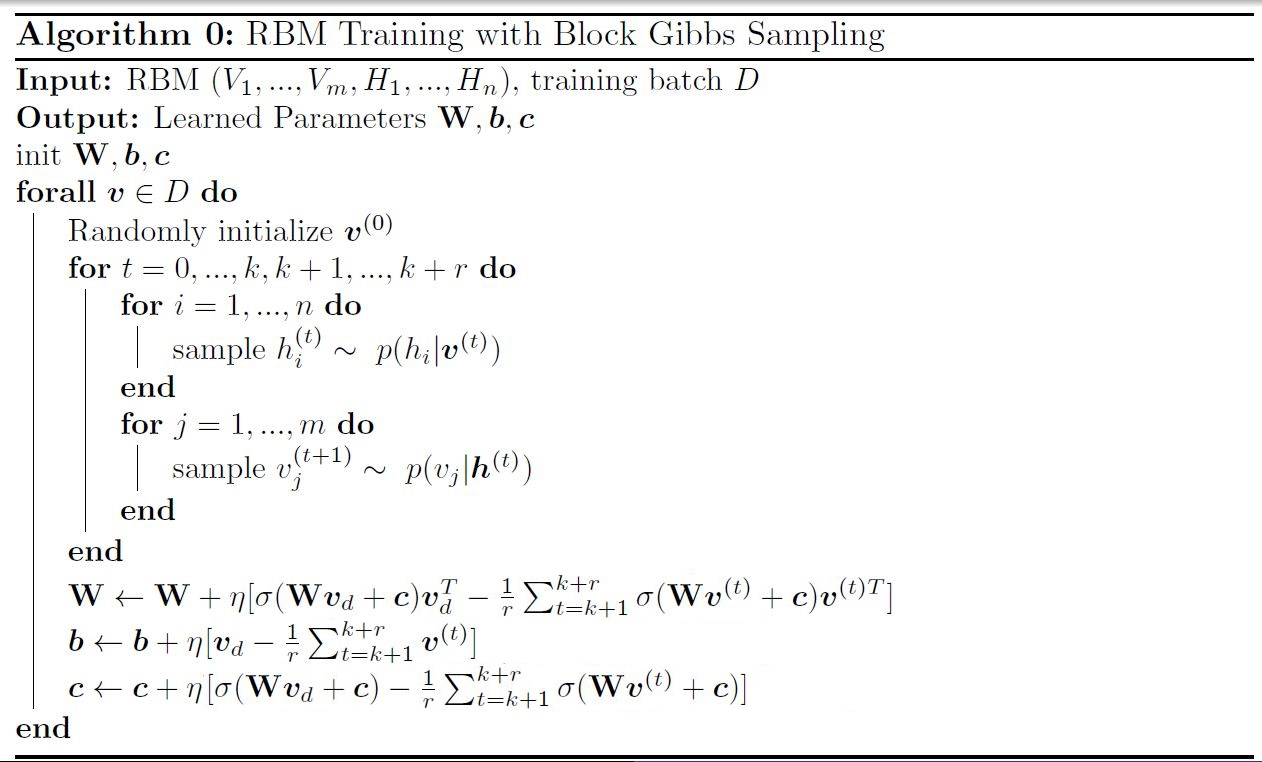
\includegraphics[scale=0.65]{Chapters/Figures/lect_20_slide_54_RBM_algorithm.JPG}
    \caption{RBM Algorithm}
    \label{fig:rbm_algo}
\end{figure}

The drawback of the Gibbs sampling based approach is that, it could take many iterations $(k)$ to reach the stationary distribution since we initialize $V^{0}$ randomly. There is an approach called k-contrastive divergence approach, where the $V^{0}$ is initialized to the current training data sample $V_{d}$ following which, the vanilla Gibbs Sampling is run. for k steps. Let the sample at the $k^{th}$ step be denoted by $\tilde{V}$(refer Fig.~\ref{fig:Conrastive_divergence}). 

\begin{figure}[h]
    \centering
    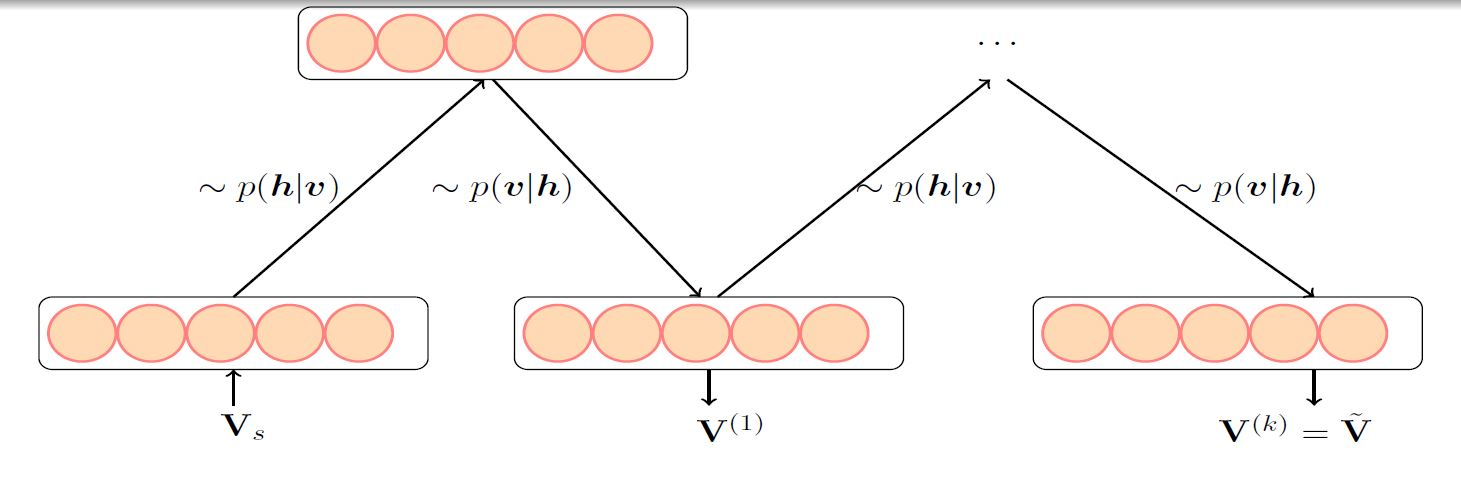
\includegraphics[scale=0.6]{Chapters/Figures/lect_20_slide_58_Conrastive_divergence.JPG}
    \caption{Contrastive divergence}
    \label{fig:Conrastive_divergence}
\end{figure}

The update rule for k-contrastive divergence approach can be written as per eq.~\ref{kcd}:
\begin{equation}
\label{kcd}
    \begin{aligned}
    W=&W+\sigma(WV_{d}+C)V_{d}^{T}-\sigma(W\tilde{V}+C)\tilde{V^{T}}\\
    b=&b+V_{d}-\tilde{V}\\
    C=&C+\sigma(WV_{d}+C)-\sigma(W\tilde{V}+C)
    \end{aligned}
\end{equation}

In practice $k=1$ is work fine. The detailed algorithm to train RBM using  k-contrastive divergence approach is depicted in Fig.~\ref{fig:Conrastive_divergence_algo}.




\begin{figure}[h]
    \centering
    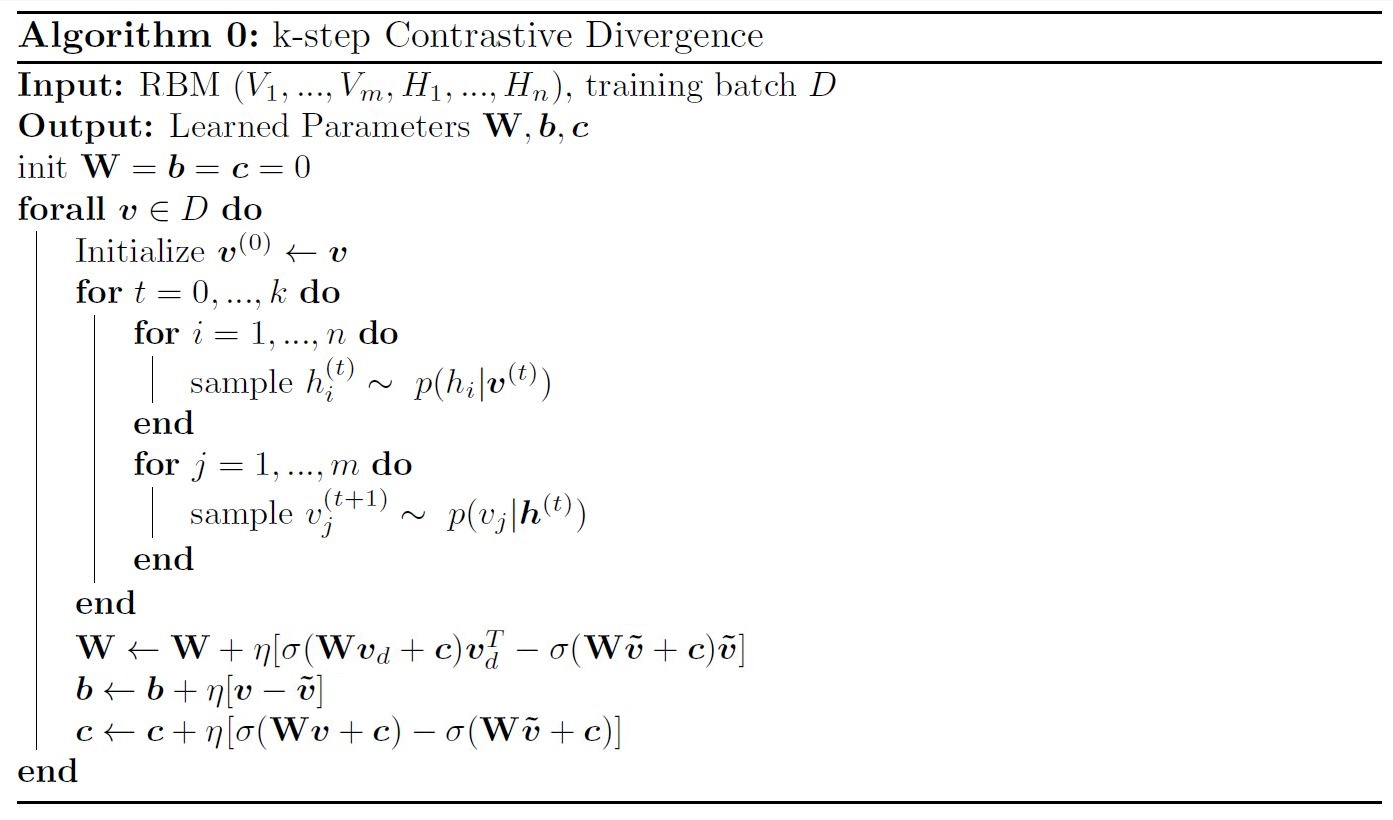
\includegraphics[scale=0.65]{Chapters/Figures/lect_20_slide_60_Conrastive_divergence_algo.JPG}
    \caption{Conrastive divergence algorithm}
    \label{fig:Conrastive_divergence_algo}
\end{figure}










\end{spacing} 

\chapter{Experiment Results and Discussions}
%\chaptermark{EM algorithm}
\HRule \\[-0.5cm] % Horizontal line
\lhead{\emph{\textbf{Chapter3:} Experiment Results and Discussions}}

%----------------------------------------------------------------------------------------
%	SECTIONS
%---------------------------------------------------------------------------------------
\begin{spacing}{0.5}
%\begin{document}
% \vspace{-5mm}
\section{Experimental Setup}
The system was built with tunable hidden layers and number of Gibbs sampling iterations (k). It has been observed that keeping $k=1$ is sufficient to gain good performance and that varying it showed no visible improvement in the plots. A binary-binary RBM has been (BB-RBM) used, to perform a pattern storage task.
% \vspace{-5mm}
\section{Database Description}
The standard MNIST handwriting dataset was used, quantised to a binary level to emulate a binary random data set of 784 dimensions.
\begin{figure}[h]
    \centering
    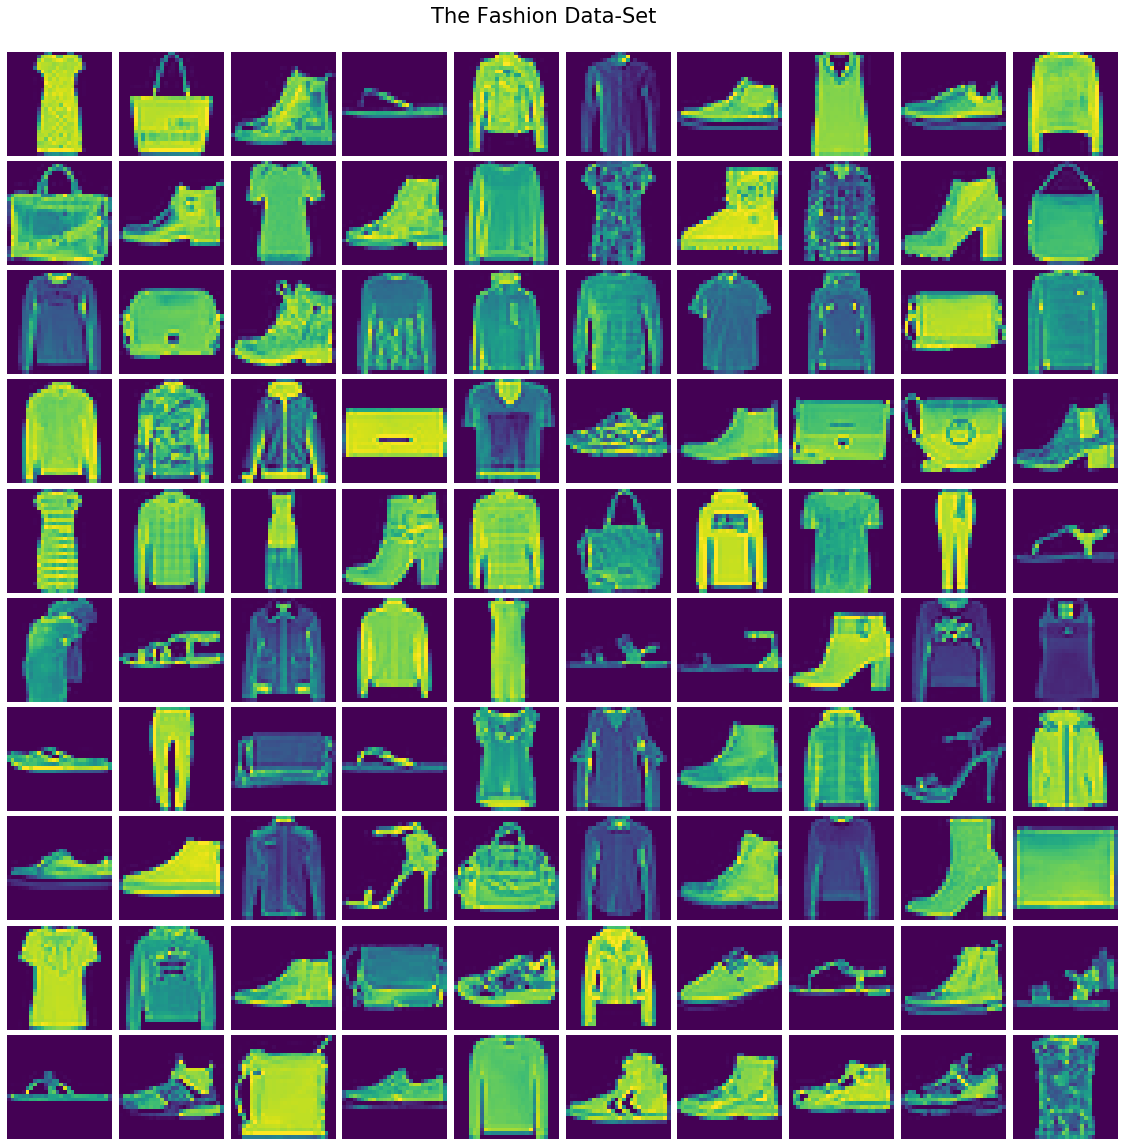
\includegraphics[scale=0.20]{Results/MNIST_DATASET.png}
    \caption{The Quantized MNIST dataset}
    \label{fig:my_label}
\end{figure}\\
\newpage
\vspace{-10mm}
\section{Results and Discussions}

\subsection{Using a 100 Hidden Layer Neurons}

\begin{figure*}[htp]
  \hspace*{-15mm}
  \subfigure[ ]{\includegraphics[scale=0.21]{Results/H_100/MNIST_348.png}}\quad
  \hspace*{+10mm}
  \subfigure[ ]{\includegraphics[scale=0.21]{Results/H_100/WEIGHTS_348.png}}

  \hspace*{-15mm}
  \subfigure[ ]{\includegraphics[scale=0.21]{Results/H_100/MNIST_FULL.png}}\quad
  \hspace*{+10mm}
  \subfigure[ ]{\includegraphics[scale=0.21]{Results/H_100/WEIGHTS_FULL.png}}
  \caption{ Figures (a) and (c) show the outputs of an RBM trained on the digits [3,4,8] and [0-9], respectively. Figures (b) and (d) show the weights between inputs and hidden layers, as an image, for these two cases.  }
\end{figure*}

\newpage

\subsection{Using 49 Hidden Layer Neurons}

\begin{figure*}[htp]
  \hspace*{-15mm}
  \subfigure[ ]{\includegraphics[scale=0.21]{Results/H_49/MNIST_348.png}}\quad
  \hspace*{+10mm}
  \subfigure[ ]{\includegraphics[scale=0.21]{Results/H_49/WEIGHTS_348.png}}

  \hspace*{-15mm}
  \subfigure[ ]{\includegraphics[scale=0.21]{Results/H_49/MNIST_FULL.png}}\quad
  \hspace*{+10mm}
  \subfigure[ ]{\includegraphics[scale=0.21]{Results/H_49/WEIGHTS_FULL.png}}
  \caption{ Figures (a) and (c) show the outputs of an RBM trained on the digits [3,4,8] and [0-9], respectively. Figures (b) and (d) show the weights between inputs and hidden layers, as an image, for these two cases.  }
\end{figure*}

\newpage

\subsection{Using 9 Hidden Layer Neurons}

\begin{figure*}[htp]
  \hspace*{-15mm}
  \subfigure[ ]{\includegraphics[scale=0.21]{Results/H_9/MNIST_348.png}}\quad
  \hspace*{+10mm}
  \subfigure[ ]{\includegraphics[scale=0.21]{Results/H_9/WEIGHTS_348.png}}

  \hspace*{-15mm}
  \subfigure[ ]{\includegraphics[scale=0.21]{Results/H_9/MNIST_FULL.png}}\quad
  \hspace*{+10mm}
  \subfigure[ ]{\includegraphics[scale=0.21]{Results/H_9/WEIGHTS_FULL.png}}
  \caption{ Figures (a) and (c) show the outputs of an RBM trained on the digits [3,4,8] and [0-9], respectively. Figures (b) and (d) show the weights between inputs and hidden layers, as an image, for these two cases.  }
\end{figure*}

% \begin{figure}[h]
%     \centering
%     \includegraphics[scale=0.20]{Results/H_100/MNIST_348.png}
%     \caption{The quantized MNIST dataset}
%     \label{fig:my_label}
% \end{figure}

% \begin{figure}[h]
%     \centering
%     \includegraphics[scale=0.20]{Results/H_100/MNIST_FULL.png}
%     \caption{The quantized MNIST dataset}
%     \label{fig:my_label}
% \end{figure}
% \section{Summary}


\end{spacing} 
% \input{Chapters/Chapter04/Chapter04}
%
\chapter{Kernel Density Estimates}
%\chaptermark{EM algorithm}
\HRule \\[-0.5cm] % Horizontal line


%----------------------------------------------------------------------------------------
%	SECTIONS
%---------------------------------------------------------------------------------------
\begin{spacing}{1.5}
%\begin{document}

\section{Kernel Density Estimates}


%\document{Kernel Density Estimates}
%\HRule \\[-0.5cm]

%\begin{spacing}[1.5]
 Kernel Density Estimation (KDE) is a non-parametric way to estimate the probability density function of a random variable.Kernel density estimation is a fundamental data smoothing problem where inferences about the population are made, based on a finite data sample.Kernel Density Estimation is also called Parzen Window.The Parzen-window approach to estimating densities can be introduced by temporarily
assuming that the region $R_{n}$ is a $d$-dimensional hypercube. If $h_{n}$ is the length of an edge of that hypercube, then its volume is given by
                                                  
                                                  
                                                 $V_{n}$=$h_{n}^{d}$
We can obtain an analytic expression for $k_{n}$, the number of samples falling in the window hypercube, by defining the following window function~\cite{parzenwindow}.
\begin{equation}
\varphi(\mathbf{u})=\left\{\begin{array}{ll}
1 & \left|u_{j}\right| \leq 1 / 2 \\
0 & \text { otherwise. }
\end{array} \quad j \neq 1, \ldots, d\right.
\end{equation}
Thus, $\varphi(u)$ defines a unit hypercube centered at the origin. It follows that $\varphi\left(\frac{x-x_{i}}{h_{n}}\right)$ is equal to unity if $x_{i}$ falls within the hypercube of volume $V_{n}$ centered at $x$, and is zero otherwise. The number of samples in this hypercube is therefore given by
\begin{equation}
k_{n}=\sum_{i=1}^{n} \varphi\left(\frac{x-x_{i}}{h_{n}}\right)
\end{equation}
\begin{equation}
p_{n}(\mathbf{x})=\frac{1}{n} \sum_{i=1}^{n} \frac{1}{V_{n}} \varphi\left(\frac{\mathbf{x}-\mathbf{x}{i}}{h_{n}}\right)
\end{equation}
In this Parzen window method, we are going to Estimate the Gaussian univarient and multivariate probability density function with different window sizes.
A Univariate Gaussion Kernel is
\begin{equation}
\varphi_{h}(u)=\frac{1}{\sqrt{2 \pi}} \exp \left[-\frac{1}{2} u^{2}\right]
\end{equation}
The resulting density is given by
\begin{equation}
p(x)=\frac{1}{n} \sum_{i=1}^{n} \frac{1}{h_{n} \sqrt{2 \pi}} \exp \left[-\frac{1}{2 h_{n}^{2}}\left(\mathrm{x}-\mathrm{x}_{i}\right)^{2}\right]
\end{equation}
It shows Parzen-window estimates of a univariate gaussian density using different window widths and number of samples. Here's the figure that I got from my MATLAB code. especially for $n$= 10, 100, 10000 with different window width $h_{1}$= 1, 0.5, 0.2
\section{Results}
\begin{figure}[h]
\label{fig:Parzen window }
  \centering
  {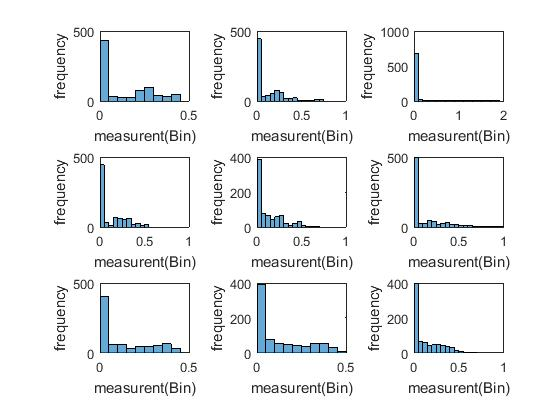
\includegraphics[scale=.7]{Images/histogram of parzen window.jpg} }
  \caption{Histogram of Parzen window estimation for different window sizes.}
\end{figure}

\begin{figure}[h]
\label{fig:Parzen window }
  \centering
  {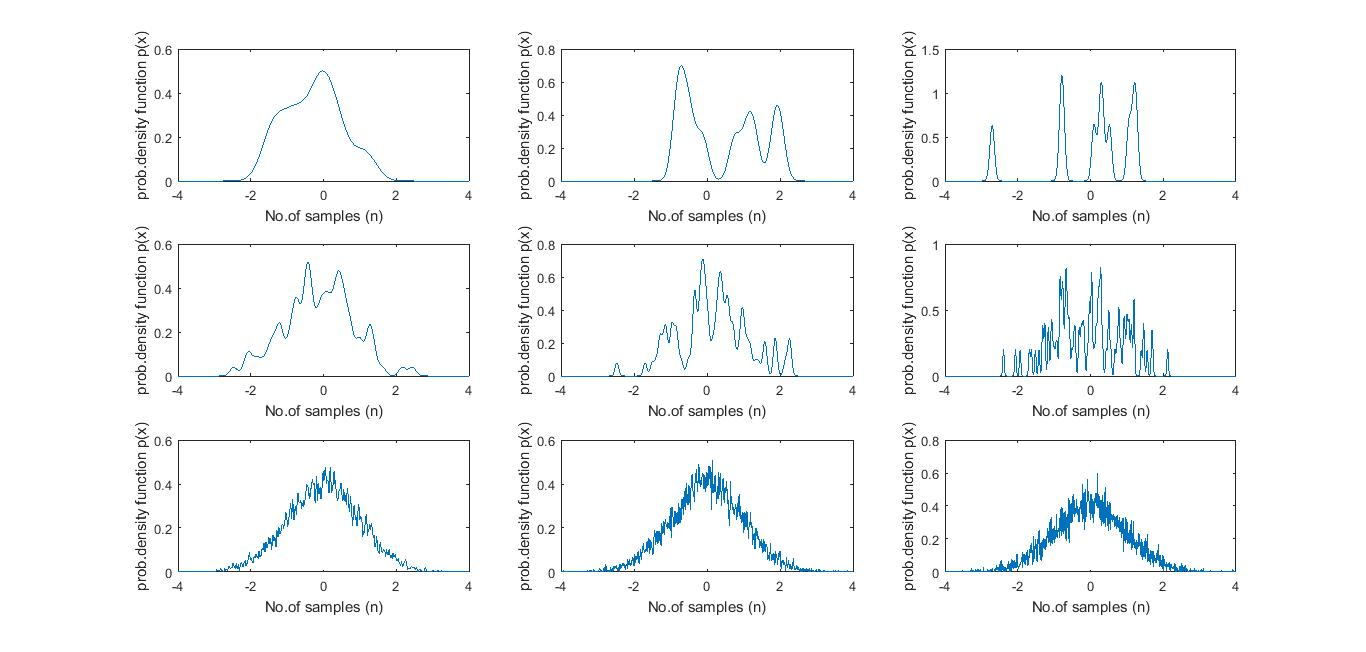
\includegraphics[scale=.38]{Images/parzen window(univarient).jpg} }
  \caption{Parzen window estimation for different window sizes.}
\end{figure}

%\end{spacing}
%\end{document}{}

\end{spacing} 
%\input{Chapters/Chapter06/Chapter06}

%----------------------------------------------------------------------------------------
%	APPENDICES
%----------------------------------------------------------------------------------------
% 
% \addtocontents{toc}{\vspace{2em}} % Add a gap in the Contents, for aesthetics
% 
% \appendix % Cue to tell LaTeX that the following 'chapters' are Appendices
% 
% % Include the appendices of the thesis as separate files from the Appendices folder
% % Uncomment the lines as you write the Appendices
% 
% % Appendix A

\chapter{Appendix Title Here} % Main appendix title

\label{AppendixA} % For referencing this appendix elsewhere, use \ref{AppendixA}

\lhead{Appendix A. \emph{Appendix Title Here}} % This is for the header on each page - perhaps a shortened title

Write your Appendix content here.
% %\input{Appendices/AppendixB}
% %\input{Appendices/AppendixC}
% 
% \addtocontents{toc}{\vspace{2em}} % Add a gap in the Contents, for aesthetics
% 
% \backmatter

%----------------------------------------------------------------------------------------
%	BIBLIOGRAPHY
%----------------------------------------------------------------------------------------
\cleardoublepage{}
\addtocontents{toc}{\vspace{1em}} % Add a gap in the Contents, for aesthetics
\clearpage % Start a new page

\label{Bibliography}
\lhead{\emph{Bibliography}} % Change the page header to say "Bibliography"
\setstretch{1}
\bibliographystyle{Bibliography/IEEEtran}
\bibliography{Bibliography/Bibliography.bib}



%%%%------------------------------------------------------List of Publications--------------------------------------------------------------------
% \cleardoublepage{}
% \addtocontents{toc}{\vspace{1em}} % Add a gap in the Contents, for aesthetics
% \clearpage % Start a new page

% \addtotoc{List of Publications}
% %\label{List of Publications}
% \lhead{\emph{List of Publications}} % Change the page header to say "Bibliography"
% \begin{center}

% \textsc{\textbf{\fontsize{24}{22}\selectfont{List of Publications}}}\\[1.0cm] % University name

% \end{center}

%
\pdfbookmark[2]{Publications}{publications}

\chaptermark{Publications}

%\section*{List of Publications/Awards/Seminars}

%\HRule \\[2cm] % Horizontal line

\label{List of Publications} % For referencing the chapter elsewhere, use \ref{Chapter1}

%\lhead{\emph{List of Publications} } % This is for the header on each page - perhaps a shortened title
%%% Please follow IEEE referencing format
%----------------------------------------------------------------------------------------
%	SECTIONS
%----------------------------------------------------------------------------------------
\begin{spacing}{1.5}


\subsection*{National and International Conferences}
\begin{itemize}
\item \textbf{Jagabandhu Mishra}, Madhusudan Singh and Debadatta Pati, \textquotedblleft{}\textbf{Processing linear prediction residual
signal to counter replay attacks},''
SPCOM-2018.

\item \textbf{Jagabandhu Mishra}, Madhusudan Singh and Debadatta Pati, \textquotedblleft{}\textbf{LP residual features to counter replay attacks},''
ICSigSys-2018.

\item \textbf{Jagabandhu Mishra}, Madhusudan Singh and Debadatta Pati, \textquotedblleft{}\textbf{Exploring linear prediction residual signal for
developing countermeasures to playback attacks},''
SCEECS-2018.

\item Madhusudan Singh, \textbf{Jagabandhu Mishra} and Debadatta Pati, \textquotedblleft{}\textbf{Development of playback attacks detection system},''
IEEE-TENCON-2017.

\item Madhusudan Singh, \textbf{Jagabandhu Mishra} and Debadatta Pati, \textquotedblleft{}\textbf{Usefulness of linear prediction residual signal for
development of replay attacks detection system},''
NCC-2017.

\item Madhusudan Singh, \textbf{Jagabandhu Mishra} and Debadatta Pati, \textquotedblleft{}\textbf{Replay attack: Its effect on GMM-UBM based
text-independent speaker verification system},''
IEEE-UPCON-2016.


\end{itemize}

% \subsection*{International Journals}
% \begin{itemize}
% \item FirstName1 LastName1 and FirstName2 LastName2, \textquotedblleft{}\textbf{Paper Title},''
% Journal Name.
% \item FirstName1 LastName1 and FirstName2 LastName2, \textquotedblleft{}\textbf{Paper Title},''
% Journal Name.
% \end{itemize}

\subsection*{Papers Submitted}
\begin{itemize}
\item \textbf{Jagabandhu Mishra}, Madhusudan Singh and Debadatta Pati, \textquotedblleft{}\textbf{Modelling glottal flow derivative signal for
detection of replay speech samples},''
NASA/ESA-AHS-2018.
% \item FirstName1 LastName1 and FirstName2 LastName2, \textquotedblleft{}\textbf{Paper Title},''
% Journalz Name.
\end{itemize}


% \subsection*{Awards/Honor/Talks}
% \begin{itemize}
% \item Award 1
% \end{itemize}
\bigskip{}


\noindent

\end{spacing} 



%%%%---------------------------------------------------------------------------------------------------------------------------------------------------------



\end{document}
